\documentclass[12pt]{article}
\usepackage{algorithm}
\usepackage{amsmath}
\usepackage{algpseudocode}
\usepackage[%
    left=1.3in,%
    right=1.3in,%
    top=1.0in,%
    bottom=1.0in,%
    paperheight=11in,%
    paperwidth=8.5in%
]{geometry}%

\usepackage[english]{babel}
\usepackage{blindtext}
\usepackage[]{hyperref}
\hypersetup{colorlinks=false,linkcolor=false,pdfborder = {0 0 0}
}
\geometry{top=2cm,bottom=2cm}
\usepackage{setspace}
\usepackage{graphicx}
\graphicspath{{images/}}
\onehalfspacing

\usepackage{pdfpages}


\usepackage[acronym]{glossaries}
\newacronym{ny}{NY}{New York}
\begin{document}
\newpage
\thispagestyle{empty}
{
\hypersetup{linkcolor=false}
\tableofcontents

}
\newpage
\pagebreak
\hspace{0pt}
\vfill
\begin{center}
\section{Introduction}
\end{center}
\vfill
\hspace{0pt}
\pagebreak

\subsection{Introduction}
These days, mobile robots have taken place in many fields like industry automation, planetary exploration, entertainment, and construction ..., for their ability to work in extreme environments with high precision and without fatigue\cite{rubio2019review}.Even so, a robot occasionally needs the support of other robots because it is impossible or difficult for them to perform some tasks on their own. For that, a new field has emmerged to deal with these problems, swarm robotics.

 
Swarm robotics is relatively a new research topic that has gained more attraction in the last few years. It is about  studying how a large number of simple robots (a swarm) can collaborate and work together to achieve predefined objectives and tasks that are often difficult or impossible to do for a single robot.\cite{bayindir2016review}.

One of the main challgenes that swarm robotics researchs face, is pattern formation. Where the agents (robots) try to form diffrent gemoetric shapes like squeres,trinagles and circles in order to perform a specific task.

We can solve this problem using two different aproches. The first one is a Centrelized method where there exist a centel unit  which controles the swarm and give global state access. However,  implementing this apporch  can be coslty and less robust to faillures. The second aproch is a dicentrilzed one, where each robot have uses local commucintion and have access only to his local state.\cite{bayindir2007review}

Our primary objective in this thesis is to implement an RL algorithm in a system made up of a group of robots in order to form some specific geometric patterns using a decentralized  method. Each robot will only have access to its local state and will interact and communicate with its neighbors in order to form the desired shapes.
 




\newpage
\pagebreak
\hspace{0pt}
\vfill
\begin{center}
\section{Swarm Robotics}
\end{center}
\vfill
\hspace{0pt}
\pagebreak




                  
\subsection{Swarm Intelligence and Social animal inspiration}
Social animal and insects behavior in groups like the bees dancing, wasp’s nest-building, ant's collaboration , bird flocking and fish schooling  has caught the attention of researchers for their ability to archive complex tasks and working in coordination, which demonstrate some form of swarm intelligence  that researchers have taken inspiration from to design and implement swarm robotics systems.\cite{navarro2013introduction} 

They also report that social insects were able to accomplish thier goals like searching for food, alerting the presence of an enemy, or collaborate to lift heavy objects, without having access to the global state or having a leader to guide them. They were only able to accomplish this by utilizing local interactions and communication, which spread to other members and and prompted group-wide cooperation.\cite{navarro2013introduction} 



\subsection{Swarm robotics and multi robot systems}
The early 1980s are when multi robots systems first gained popularity.
As the name suggests, multi robot systems introduce the idea of teamwork in order to complete tasks that are challenging or impossible to complete alone by the robots.
Seven topics of study have been identified in this feild which includes:
\begin{itemize}
  \item  Biological Inspirations; 
  \item Communication
  \item Localization, mapping, and exploration;
  \item Object transport and manipulation;
  \item Motion coordination; 
  \item Reconfigurable robots.
\end{itemize}
Swarm robotics is a subfield of multi-robot systems that differs from other multi-robot systems in some ways.\cite{arai2002advances}
   


 

\subsection{Swarm robotics}
Swarm robotics has no one definition because it is a rapidly developing area and new research is constantly being done in it. But we can take this defintion from a cited paper.
"swarm robotics is the study of how large number of relatively simple physically embodied agents can be
designed such that a desired collective behavior emerges from the local interactions among agents
and between the agents and the environment."\cite{csahin2005swarm}.\\

The main characters of swarm robotis are:
\begin{itemize}
  \item  The robots in the swarm must be autonomous. 
  \item The number of robots in the swarm is large.
  \item Homogeneity is required in robots. A small number is acceptable if not.
  \item Robots must be incompetent  with regard to the primary task they must complete, otherwise, they will fail or perform poorly.
  \item Robots are limited to local communication and sensing. It makes sure that coordination is spread, making scalability one of the system's characteristics.\cite{navarro2013introduction}
\end{itemize}


\subsection{Swarm robotics properties}
Swarm robotics have some properties that describe the system's current condition. Bellow are some of these properties:

\textbf{Robustness}: the ability of the swarm to  still function even with the loss of some members of the group or the faillure of some parts of the system.\\
\textbf{Scalability}: The ability of the system to perform well on smaller or larger group sizes without impacting the performance of the swarm.

\textbf{Flexibility} It is the capability of the swarm to adapt and manage the new changes that occur in the environment 

\textbf{Autonomus}: Implys that there is no central authority controlling the behavior of the swarm and each individual is independent of the others.

\textbf{Local communication} The communication among swarm members is local since they don't have access to  the swarm's overall state.
\cite{brambilla2013swarm}\cite{olaronke2020systematic} 

  

\subsection{Domain of application}
In this section, we will list some of the significant fields domains where swarm robotics fits in, and can impact in solving the domain problem.\newpage
\subsubsection{Tasks that cover a region}:
Because of the widespread sensing capabilities that the swarm has, swarm robotics is most suited for tackling problems that cover an area of the space, such monitoring the environment of a lake or  surveillance of a specific area.\cite{csahin2005swarm}\cite{olaronke2020systematic}

\subsubsection{Search and rescue missions}
In different types of accident or disasters that happen like earthquakes where the human intervention is difficult, swarm robots can be deployed for these type of missions. examples of such robots are: polyobot, swarm bot and M-TRAN.

\subsubsection{Cleaning of oil speals}
A swarm of robots can reduce the cost and time in such incidents. an exemple of robots that were deployed to such tasks is: Seaswarm, which was developed by the senseable group at MIT.

\subsubsection{Exploration}
To investigate Mars, swarm robots like Marsbees have been created. the same holds true for the CoCoRo swarm, which was employed for in-depth underwater investigation.
\subsubsection{Agriculture}
As they can be used to improve the agriculture and monitor the status of crops. 

\subsection{Swarm robotics basic tasks and problems}
SR problems can be broken down into fundamental tasks that the swarm frequently carries out in an effort to accomplish its objective.
this tasks are: aggregation,d ispersion,pattern formation, coordinated
movement, hole avoidance and foraging\cite{bayindir2007review}\cite{navarro2013introduction}.
\newpage
\subsubsection{Aggregation}
Aggregation of the robots is performed in order to accomplish some form or to exchange information. This problem can be easy in a centralized system, but  difficult in a decentralized one.
\subsubsection{Dispersion}
For exploration purposes, sometimes, the swarm must cover a wide range of area without losing the connection between the members, in order to expand the group sensing capabilities. 

\subsubsection{Pattern formation}
Sometimes, the swarm must form some specific patterns like circles,squares or  lines in order to lift some objects or traverse some ways corridors.
\subsubsection{Cordinated movement}
It is making an effort to coordinate the group movements by maintaining the established pattern between the robots.
\subsubsection{Hole avoidance}
As suggested by the name, the group makes an effort to avoid stepping into holes.
\subsubsection{Foraging}
The swarm aims to locate objects, pick them up, and position them where needed.

\newpage
\pagebreak
\hspace{0pt}
\vfill
\begin{center}
\section{Deep reinforcement learning}
\end{center}
\vfill
\hspace{0pt}

\pagebreak

\subsection{Introduction}
In this chapter we will provide an overview about the feild of reinforcement learning, including its applications, various techniques, and how it relates to swarm robots.\\
Before that,we will briefly discuss machine learning since it is the foundation of RL before we move on.
\subsection{Machine learning}
Machine learning is a sub field of artificial intelligence, which
focuses on developing algorithms and models that make prediction and take decisions without being explicitly programmed to do so
based on the input data they receive.
Generally speaking, there are three types of machine learning algorithms,
suppervised algorithms which obtain labeled data and attempt to categorize or anticipate the unknown one. Unsupervised learning algorithms, where the  data is unlabeled and it is the job of the ml algorithms  to extract  hidden patterns in it. And finally, reinforcement learning algorithms  where the algorithm learns to make decisions based on trial and error and rewards, by interacting with an environment.
  
\subsection{Reinforcement learning}
Reinforcement learning algorithms are based on a agent that interact and observe  an environment in order to take actions that maximize the reward for a given task.

The goal of the agent is to learn an optimal policy ($\Pi$) which maps state to actions in order to get the best possible action to take in a given situation. This can be achieved  by maximizing the expected  reward that the agent receive from the environment on each step he takes.\cite{arulkumaran2017brief}

Formally, RL can be described as a Markov Decision Process (MPD) where the future state depends only on the current one. An MPD  consists of:

\begin{itemize}
  \item  A set of states $S$
  \item  A set of actions $A$
  \item  A transition dynamics $\rho(S_{t+1}|a,S)$. which give the probability of being in state $S_{t+1}$ based on the current state $S$ and the performed action $A$.
  \item A reward function $R(S_{t},A_{t},S_{t+1})$ which outputs a scalar reward $r_{t} \subset R$. 
   \item A discount factor $\gamma \in [0,1]$ which  emphasis either  immediate or future rewards.
\end{itemize}

\newpage
From the above definition, the policy function $\Pi$ will  a map a given state to a probabilty distribution over actions: $\Pi: S \longrightarrow \rho(A=a|S)$.
The goal of the agent to find the optimal policy $\Pi$ which maximize the expected return :\\
\[ \Pi^{*} = argmax_{\Pi}  E[R|\pi] \]

If the MPD is episodic, then the agent will accumulates a set of reward at the end of each episode which is called a return:

\[ R= \sum_{t=0}^{T-1} \gamma^{t}r_{t+1} \]

Setting $\gamma<1$ will ensure the convergence of the return in case of non episodic MPDS.\cite{arulkumaran2017brief}.

\subsection{Q learning}
Q-learning is a type of model free reinforcement learning algorithm  based on the dynamic programming technique, where the agent tries to maximize it rewards by finding the optimale policy $\Pi$ in an iterative manner. In order to  acheive this, the agent uses a type of equation called value function that gives it the value or the reward of being in a state $s$ and taking action according to it policy $\Pi$.


\[ V^{\Pi}(S)=E[r(s,a)+\gamma V^{\Pi}(s') ] \] 

In order to find the optimal value function, hence finding the optimal policy, the equation must satisty the bellman optimality condition which states that: 

  
\[ V^{*}(S)=max_{a}E[r(s,a)+\gamma V^{*}(s') ] \] 

The same goes for the action-value function which gives the return if the agent chooses the action $a$ and follow the optimale policy thereafter.

\[ Q^{*}(S,a)=E[r(s,a)+max_{a}\gamma Q^{*}(s',a) ] \]\cite{watkins1992q}.


\pagebreak

\subsection{Deep Q learning}
The problem with traditional Q-learning or Rl algorithms in general, is the inability to work in  a high dimensional input states where discritization and hand-crafted features extraction    is performed in order to it to work. For this, deep learning was combined with traditional Q-learning in order to overcome these challenges.\cite{mnih2013playing}

Deep Q learning was firstly introduced in an article by the deepmind group, where it was tested in atari games in which the agent was given raw input images of the emulator and it was the  goal of the agents to win the games by using the Q learning algorithm.

Besides using the bellmen equation to converge and calculate the loss, an experience replay memory was used to store the the experiences of the agents during  the game and then sampled randomly to be  fed to the neural network to learn and in order to break the correlation that apears when fedding them sequential data.\cite{mnih2013playing}
 
\begin{algorithm}
\caption{Deep Q-learning with Experience Replay}\label{alg:cap}
\begin{algorithmic}
\State Initialize replay memory D to capacity N
\State Initialize action-value function Q with random weights
\For{\texttt{episode = 1, M}}
        \State \texttt{Initialise sequence s1 = \{x1\} and preprocessed sequenced $\phi_{1}$ = $\phi(s_{1})$  }
        \For{\texttt{t = 1, T}}
         \State With probability $\epsilon$ select a random action $a_{t}$
         \State otherwise select  $a_{t}$ = $max_{a} Q^{*}(\phi(s_{t},a;\theta) $ 
         \State Execute action $a_{t}$ in emulator and observe reward ${r_{t}}$ and image $x_{t+1}$
        \State Set $s_{t+1}$ = $s_{t}$ , $a_{t}$ , $x_{t+1}$ and preprocess  
        $\phi_{t+1}=\phi(s_{t+1})$
        \State Store transition $(\phi_{t} , a_{t} , r_{t} , \phi_{t+1} )$ in $D$
        \State Sample random
minibatch of transitions $(\phi_{t} , a_{t} , r_{t} , \phi_{t+1} )$ in $D$
        \State set  \begin{equation}
  y_{j}=\begin{cases}
    r_{j}, & \text{for terminal $\phi_{j+1} $}.\\
    r_{j}+\gamma max_{a}Q(\phi_{j+1},a';\theta) , & \text{for non-terminal $Q(\phi_{j+1})$}.
  \end{cases}
\end{equation}
        \State Perform a gradient descent step on $(y_{j} - Q(\phi_{j} , a_{j} ; \theta))$ 
        \EndFor 
\EndFor 


\end{algorithmic}
\end{algorithm}
 

 
 
algo1:
  -the leader robot or first robot will calculate the points and choose one
  and give it to hi neigbor
  -the neighbor will do the same and choose one and pass the array to the next.
  
  
  
\newpage
\pagebreak
\hspace{0pt}
\vfill
\begin{center}
\section{Problem formulation And Solution Conception }
\end{center}
\vfill
\hspace{0pt}

\pagebreak

 

\subsection{Introduction}
 In this section, we'll go into  detail about the objective that needs to be accomplished by our robots, the difficulties they must overcome, and then our suggested solution.
 
\subsection{Goal defintion}:
Our objective in this thesis is to make multi robots  form geometric patterns like lines, circles, squares, and triangles while avoiding collisions and moving toward their destination in a quick and efficient manner. 



\subsection{Problem Formulation}
 

\subsubsection{Environement}
Consider a scenario in which there are n (n> 2) robots moving in a 2D environment. Assuming that every robot is aware of a central point that they must form shapes around or along it.


 
 \begin{figure}[h]  
\centering
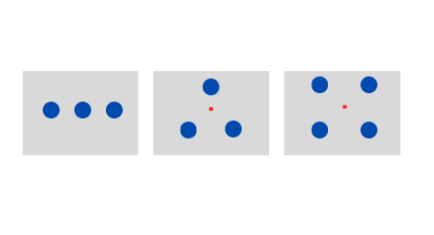
\includegraphics[scale=0.4]{formation}
\caption[formation]{formation}
\end{figure}














\subsection{State Of the art}
\subsection{DQN}
\subsection{DDPG}
\subsection{Thier usages in multi agent pros and cons}
\subsection{problem formulation and solution}
\subsection{we opt for maddpg decentrilzed excution }
\subsection{we opt for maddpg for better perfomance and scalability }


\subsection{ROS and gazebo}


\subsection{Conception of the solution}


\subsection{implemtation of the solution}











 


\newpage
\bibliography{bib}
\bibliographystyle{ieeetr}



\end{document}